%=========================================================================
% (c) Michal Bidlo, Bohuslav Křena, 2008

\chapter{Úvod}
S rozšírením a nárastom užívania moderných technológií v novom miléniu sa stala otázka bezpečnosti čoraz dôležitejšou. V minulosti bola ochrana informácií zaručená tažkou fyzickou dostupnosťou informačných systémov obsahujúcich dôležité (osobné, firemné, štátne, armádne, tajné, atď.) informácie alebo boli chránené predovšetkým sieťové prístupy do daných systémov.

V súčasnosti je digitálna ochrana fyzického prístupu k zariadeniam obsahujúcim informácie čoraz dôležitejšia, keďže ich masové rozšírenie priamo súvisí s ľahším fyzickým prístupom k nim. Zariadenia obsahujúce citlivé údaje sú s nami každý deň a na každom kroku. Zanechávame ich na verejných miestach (stoloch, lavičkách, v taškách, batohoch, atp.), často ľahko dostupné a bez dostatočného zabezpečenia.

Výrobcovia zariadení sa snažia ponúknuť svojim zákazníkom čoraz sofistikovanejšie spôsoby zabezpečenia zariadení s minimálnym dopadom na pohodlie užívateľa. Heslá, PIN-y a znakové zabezpečenie sa snažia uľahčiť zadávanie vstupného kódu avšak v mnohých prípadoch vedú k dočasnému alebo trvalému zablokovaniu prístupu k zariadeniu z dôvodu zabudnutia vstupného hesla/kódu. Z tohoto dôvodu mnohý výrobcovia presadzujú senzory, ktoré snímajú biometriu užívateľa a tak využívajú prirodzenú komplexitu ľudskej fyziológie k zabezpečeniu zariadení.

V súčasnosti je štandardom v rôznych zariadeniach snímač odtlačku prstu. Táto technológia, aj napriek viacerým zlepšeniam a detekcii živosti prstu, je stále použiteľná len pre jednoduché zabezpečenie. Prístup k odtlačkom prstov je možný aj bez vedomia vlastníka, kedže odtlačky prstov bežne zanechávajú stopu na rôznych povrchoch. Obdobným spôsobom sú vystavené verejnosti aj iné časti ľudského tela, ktoré sú používané v biometrii (napr. naše ruky, tvár, dúhovka, atp.), čo ruku v ruke s najmodernejšími snímacími technológiami smeruje k zníženej schopnosti týchto prvkov ochrániť naše dáta.

Jediným prvkom využívaným (zatiaľ len okrajovo) v biometrii, ktorý je v bežnom živote dostatočne chránený, je sietnica. Bez priameho prístupu k oku vlastníka je takmer nezaznamenateľná a teda ideálne chránená pre potreby biometrie. Bohužial, táto jej vlastnosť má aj svoju daň v podobe zníženého komfortu užívateľa pri jej snímaní.
Samotné snímanie sietnice produkuje konzistentné výsledky vďaka jej polohe v uzatvorenom priestore očnej bulvy, kde sú podmienky snímania konštantné. K zmene podmienok snímania môže dôjsť len zmenou prostredia v očnej bulve alebo zmenou sietnice samotnej. Toto býva typicky spôsobené rôznymi chorobami orgánu oka.

Táto práca sa snaží o korekciu druhého z uvedených problémov. V kapitole \ref{ch:kap0} je podaný teoretický základ biometrických metód, ako aj spôsob vyhodnocovania ich spoľahlivosti. Kapitola \ref{ch:kap1} predkladá pojmy súvisiace so zrakovým orgánom, predovšetkým sietnicou. V kapitole \ref{ch:kap2} su rozobrané jednotlivé patologické nálezy zrakového orgánu so zameraním na tie, ktoré majú najväčší dopad na snímanie sietnice. Kapitola \ref{ch:kap3} popisuje rôzne zdroje dát snímkov sietnice použité k štúdiu patologických úkazov, ich parametre a použitie pre potreby tejto práce. V kapitole \ref{ch:kap4} je pre vybrané patologické nálezy rozpracovaný teoretický podklad a spôsob akým by bolo možné dané nálezy v snímkach sietnice korigovať. Kapitola \ref{ch:kap4} ďalej prezentuje algoritmus využitý na korekciu daných nálezov vo snímkoch s ohľadom na použitie daných snímok pre účely biometrie. Kapitola \ref{ch:kap5} následne prezentuje výsledky testovania algoritmu na vybraných zdrojoch dát. Záverečná kapitola sumarizuje výsledky a predkladá ďalšie možné kroky, ktoré by mohli zlepšiť výsledky algoritmu.

\chapter{Biometria obecne}\label{ch:kap0}
\emph{Biometria} je metóda automatického rozpoznávania ľudí na základe anatomických (odtlačky prstov, tvár, dúhovka, sietnica,\dots) alebo behaviorálnych (hlas/reč, gestikulácia, chôdza, podpis,\dots) vlastností jedinečných pre každého človeka.

Kombinácia týchto vlastností predstavuje \emph{identitu}, ktorá jednoznačne určuje danú osobu. Osoba tak môže byť identická len sama so sebou\cite{bio}.

Identitu rozlišujeme:
\begin{itemize}
\item fyzickú -- 
\item elektronickú -- 
\end{itemize}

Vstupom pre biometrický systém je súhrn elektronických identít osôb, ktoré chceme rozlíšiť a identifikovať pomocou biometrického systému.

\chapter{Orgán zraku}\label{ch:kap1}
Orgán zraku je primárny párový senzorický orgán ľudského tela, vďaka ktorému sa človek dokáže jednoducho orientovať v okolitom priestore. Strategické umiestnenie tohoto orgánu na hlave (blízko mozgu) ho robí ľahko dostupným pre použitie v biometrii.

Táto kapitola rozoberá základné poznatky týkajúce sa orgánu zraku, rozoberá jeho optické vlastnosti a zavádza pojmy, ktoré sú využívané v nasledujúcich kapitolách.

\section{Zloženie oka}\label{sec:oko}
Oko, očná bulva, má takmer sférický tvar. Vďaka tomuto tvaru je jeho pohyb v očnej jamke rýchly a zabezpečuje zameranie sa na objekt záujmu v ráde milisekúnd\cite{}.
Zloženie oka umožňuje jednoduchý priestup svetla, obmedzenie množstva svetla v prípade zvýšeného jasu a jeho zaostrenie na sietnicu.

\begin{figure}[h]
  \centering
  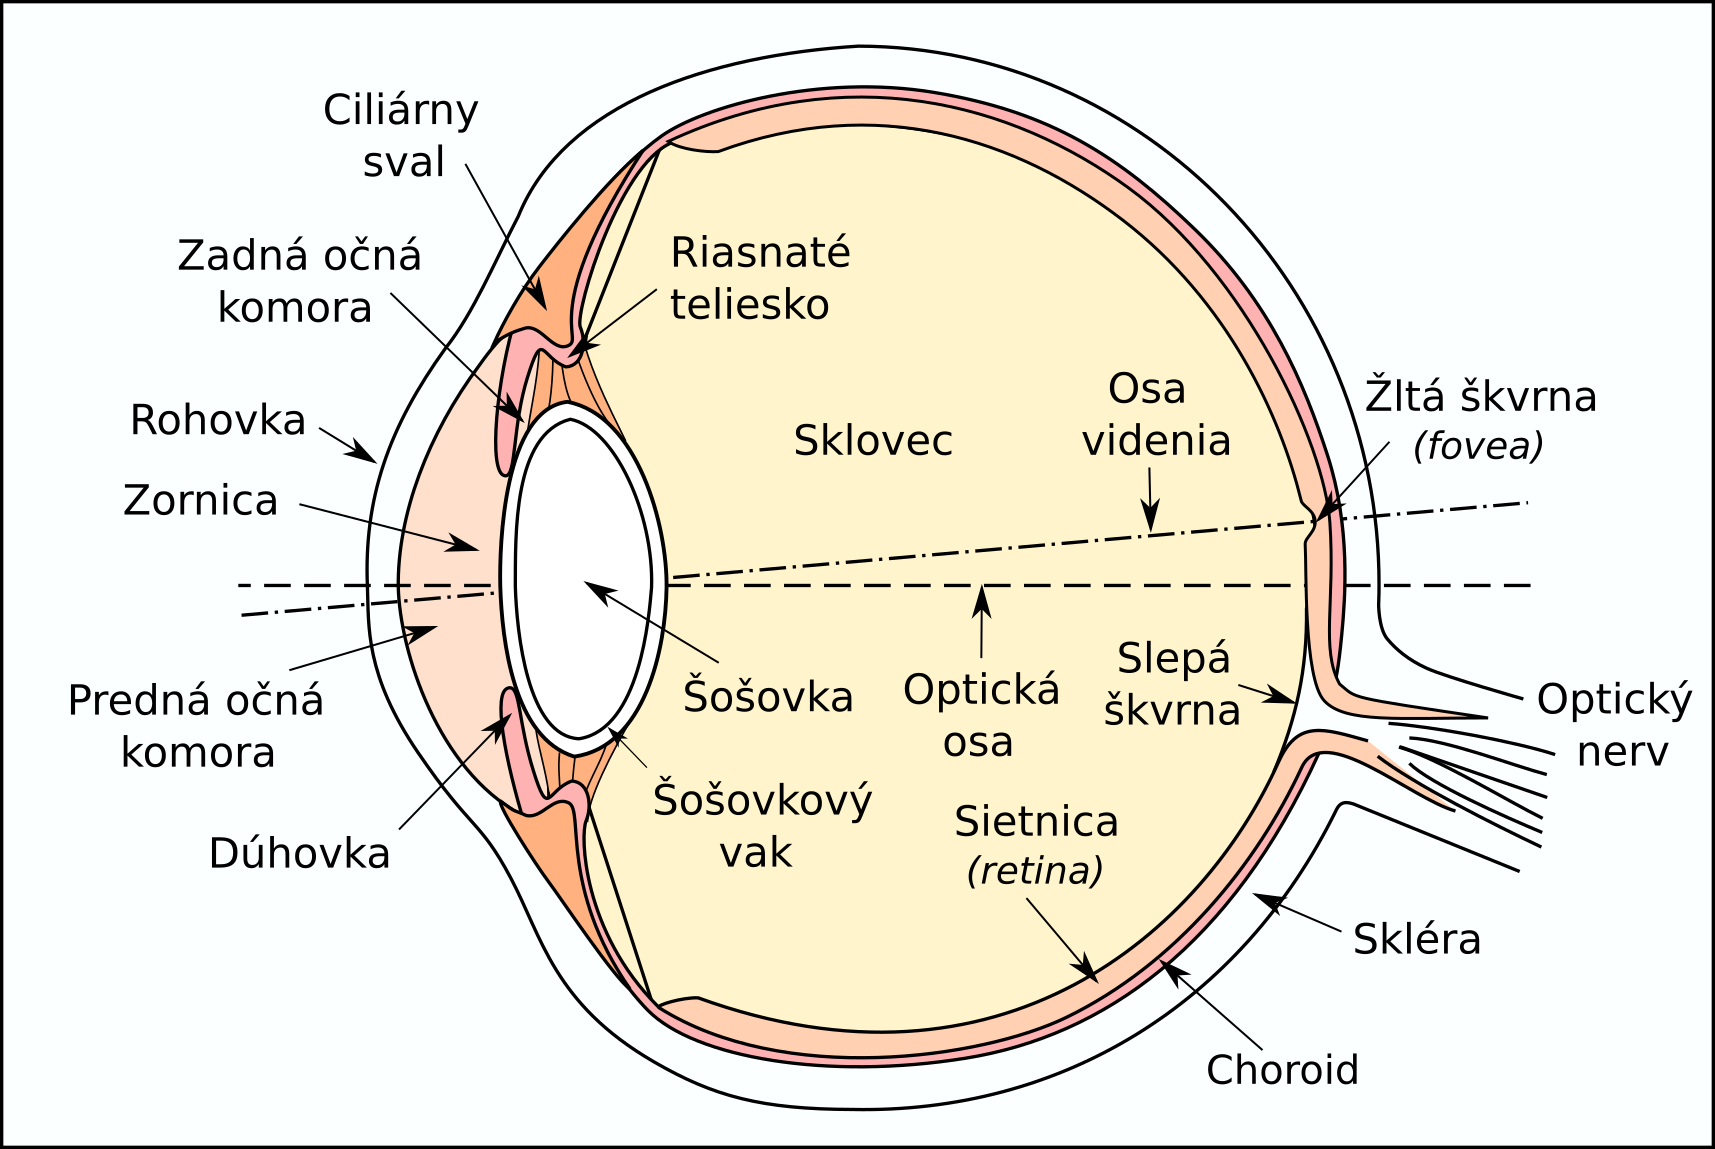
\includegraphics[width=11cm]{img/Eyesection.png}
  \caption{Štruktúra ľudského oka\cite{retina}}
\end{figure}

Svetlo pri priechode okom prechádza nasledujúcimi prvkami\cite{zloz_oka}:
\begin{itemize}
\item \textbf{rohovka} (cornea) -- transparentná vrstva v prednej časti oka chrániaca miesto vstupu svetla do oka. Je vysoko odolná a má značné regeneračné vlastnosti.
\item \textbf{predná a zadná očná komora} -- obsahujú číru tekutinu, ktorá vypĺňa priestor za rohovkou až k dúhovke a šošovke (v mieste zornice). Udržujú stály očný tlak, zásobujú rohovku, šošovku a okolité tkanivá živinami\cite{zmysly}.
\item \textbf{šošovka} -- elastický útvar bikonvexného tvaru. Je zavesená na tenkých vláknach a napínaná ciliárnym svalom, ktorý tak upravuje optickú mohutnosť šošovky a umožňuje zaostrovanie, akomodáciu.
\item \textbf{sklovec} -- číry gél vypĺňajúci dutinu oka za šošovkou.
\item \textbf{sietnica} (retina) -- viacvrstvá štruktúra obsahujúca svetlocitlivé bunky. Elektrický impulz generovaný svetlocitlivými bunkami je prenášaný sieťou komplexných nervových dráh až do mozgu.
\end{itemize}

Každý z týchto prvkov má vlastnosti, ktoré sa podieľajú na správnom prenose svetla k sietnici. 


- popis ako je svetlo ovplyvnene prvkami oka
- popis ako sa obraz dostava na sietnicu

- popis kde je sietnica a na co sluzi \cite{vlast_oka}
- potrebujes sa dostat k popisu klucovych prvkov sietnice

- 

- jednotlive casti oka a ich nazov podla odbornej literatury
- popis priepustnosti svetla skrz oko a vlastnosti svetla ktore zachytava sietnica
- odkaz na choroby ktore niesu spojene priamo so sietnicou?

\section{Sietnica}\label{sec:sietnica}
- skladba sietnice, rieciste, svetlocitlive bunky, popis jednotlivych prvkov na sietnici
- reakcia svetlocitlivych buniek na svetlo, ich rozlozenie po sietnici
- 

\section{Biometria sietnice}\label{sec:bioret}

\chapter{Patológia sietnice}\label{ch:kap2}
TBD\cite{prim}
\section{TBD}
TBD\cite{sec}
TBD\cite{bio}

\chapter{Zdroje vstupných dát}\label{ch:kap3}

\chapter{Detekcia a korekcie nálezov}\label{ch:kap4}

\chapter{Implementácia algoritmu}

\chapter{Systém testovania a výsledky}\label{ch:kap5}

\chapter{Záver}\label{ch:kap6}
Závěrečná kapitola obsahuje zhodnocení dosažených výsledků se zvlášť vyznačeným vlastním přínosem studenta. Povinně se zde objeví i zhodnocení z pohledu dalšího vývoje projektu, student uvede náměty vycházející ze zkušeností s řešeným projektem a uvede rovněž návaznosti na právě dokončené projekty.

%=========================================================================
